\chapter{NetFlow}
\label{chp:netflow}

\section{Format}
The traffic data provided by UNINETT is stored in the NetFlow File Format~\cite{cisco0netflow}.
This format consists of flows, which are data units consisting of information from the \gls{network layer} and \gls{transport layer},
 for example IP addresses, transport protocol, and port numbers where applicable.
NetFlow can be converted to human readable text using the \verb"nfdump" program\footnote{\url{http://nfdump.sourceforge.net}}.

\section{Available information}
%Apart from multicast and broadcast flows, flows are always between two hosts.
%The NetFlow information is logged by UNINETT's core routers, so only traffic that passes through these core routers is logged.
%Flows that are not logged are (1) communication in LANs and (2) communication on the open internet between hosts that have no affiliation with UNINETT.
%This means that (1) spreading of malware within a LAN, or organisation, is not detected and neither is (2) malware spreading on the internet outside of the Norwegian academic institutions.
%
%Using a list of IP addresses assigned to UNINETT and organisations peering through UNINETT, it is possible to know which hosts can be well observed (all communication with the internet is observed) and which %hosts cannot be well observed (only communication with a well observed host is observed).
%The thesis focuses mainly on hosts that can be well observed.
%
%\subsection{Observable traffic}
NetFlow data is logged on the core routers, which means that only traffic that passes through these routers is observable.
UNINETT peers with most Norwegian education institutions, which have their own routers connected to the core routers.
This means that UNINETT can only observe traffic that happens between institutions, or between institutions and hosts on the outside.
In other words, traffic between hosts within an institution is not observable for UNINETT.
%Although there exists malware with very specific targets~\cite{langner2011stuxnet}, most known malware targets any vulnerable host on the internet it can find.
%Because of this, it is expected that most malware traffic will be observable from the NetFlow data.

Figure~\ref{fig:nodes} shows some hosts in different networks, and some flows between them.
The figure illustrates how only flows that go through UNINETT's core routers will show up in the NetFlow log.
Flows between hosts within an institution will never pass through UNINETT's core routers, even though the institution is connected to the internet through UNINETT.
Flows completely outside of UNINETT's core network are not logged either, naturally.
Flows that are between one host at an institution connected through UNINETT -- for example \gls{ntnu} -- and one host in another institution, can be logged by UNINETT's core routers, because the traffic must pass through these routers.

\begin{figure}[h]
	\caption{Illustration of which flows are logged}
	\label{fig:nodes}
	\centering
		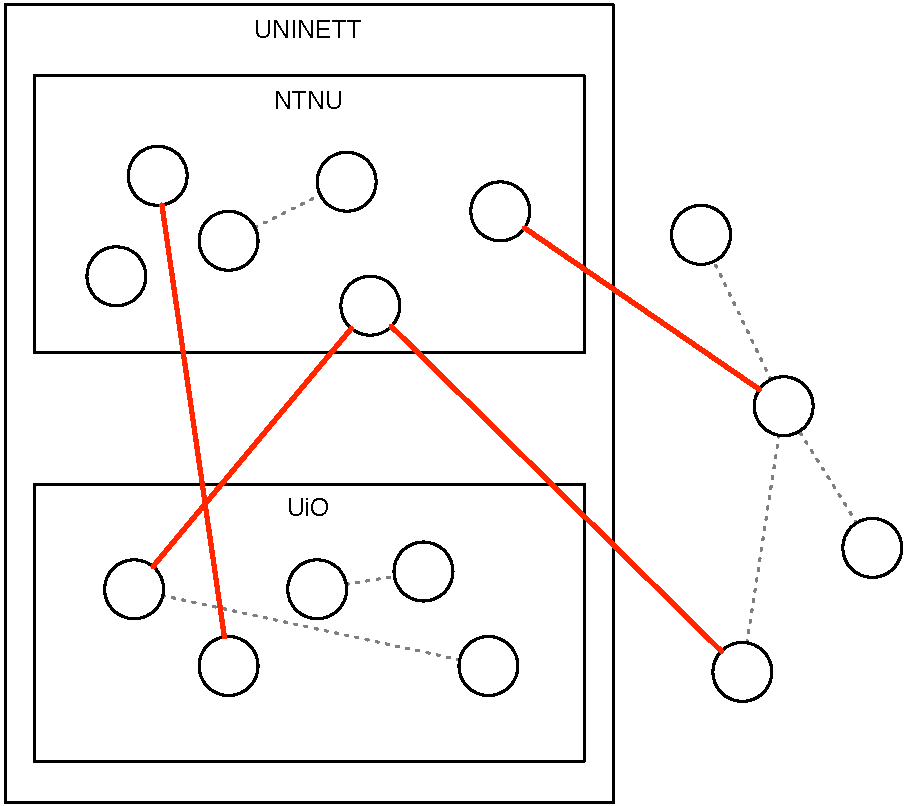
\includegraphics[width=0.5\textwidth]{nodes}
\end{figure}


\section{Direction}
\label{sec:direction}

Flows are between a source and destination IP address.
One TCP or UDP session will usually be observed as multiple flows,
because NetFlow logs are written by core routers operating on the \gls{network layer},
 which will not keep track of TCP of UDP connections, as this is a \gls{transport layer} function.
In order to observe spreading, it is important to know which host initiated the connection.
A possible solution would be to take the first flow between two hosts, and merge it with all subsequent flows that are between the same IP addresses and port numbers,
 until a time-out occurs.
However, for performance reasons, UNINETT makes use of sampled NetFlow data, which means that only 1~\% of all the packets are logged.
This makes it harder to reliably establish which party initiated a connection,
 as the first observed flow may be in the opposite direction from the actual first flow.

TCP and UDP are transport protocols which offer end-to-end communication between hosts.
In order to allow hosts to run multiple services, these protocols use a two byte \emph{port number} to indicate the type of service.
In order to set up a TCP or UDP connection, a client must first select a port number at random.
This port is called the \emph{\gls{ephemeral port}}, and its range differs per operating system, but it is never lower than 1024.
The client will then send an initial packet to the server, from the \emph{\gls{ephemeral port}}, to the \emph{\gls{contact port}}.
The \emph{\gls{contact port}} will often be a \emph{\gls{well-known port}}, which is a port number under 1024.
The direction of a flow can therefore be assumed to be initiated by the party with the lowest port number.
The list of \gls{well-known port}s is maintained by IANA~\cite{rfc1700}.


